
\section*{Supplement}

\setcounter{figure}{0}
\makeatletter 
\renewcommand{\thefigure}{S\@arabic\c@figure}
\makeatother

\begin{figure}
  \begin{center}
    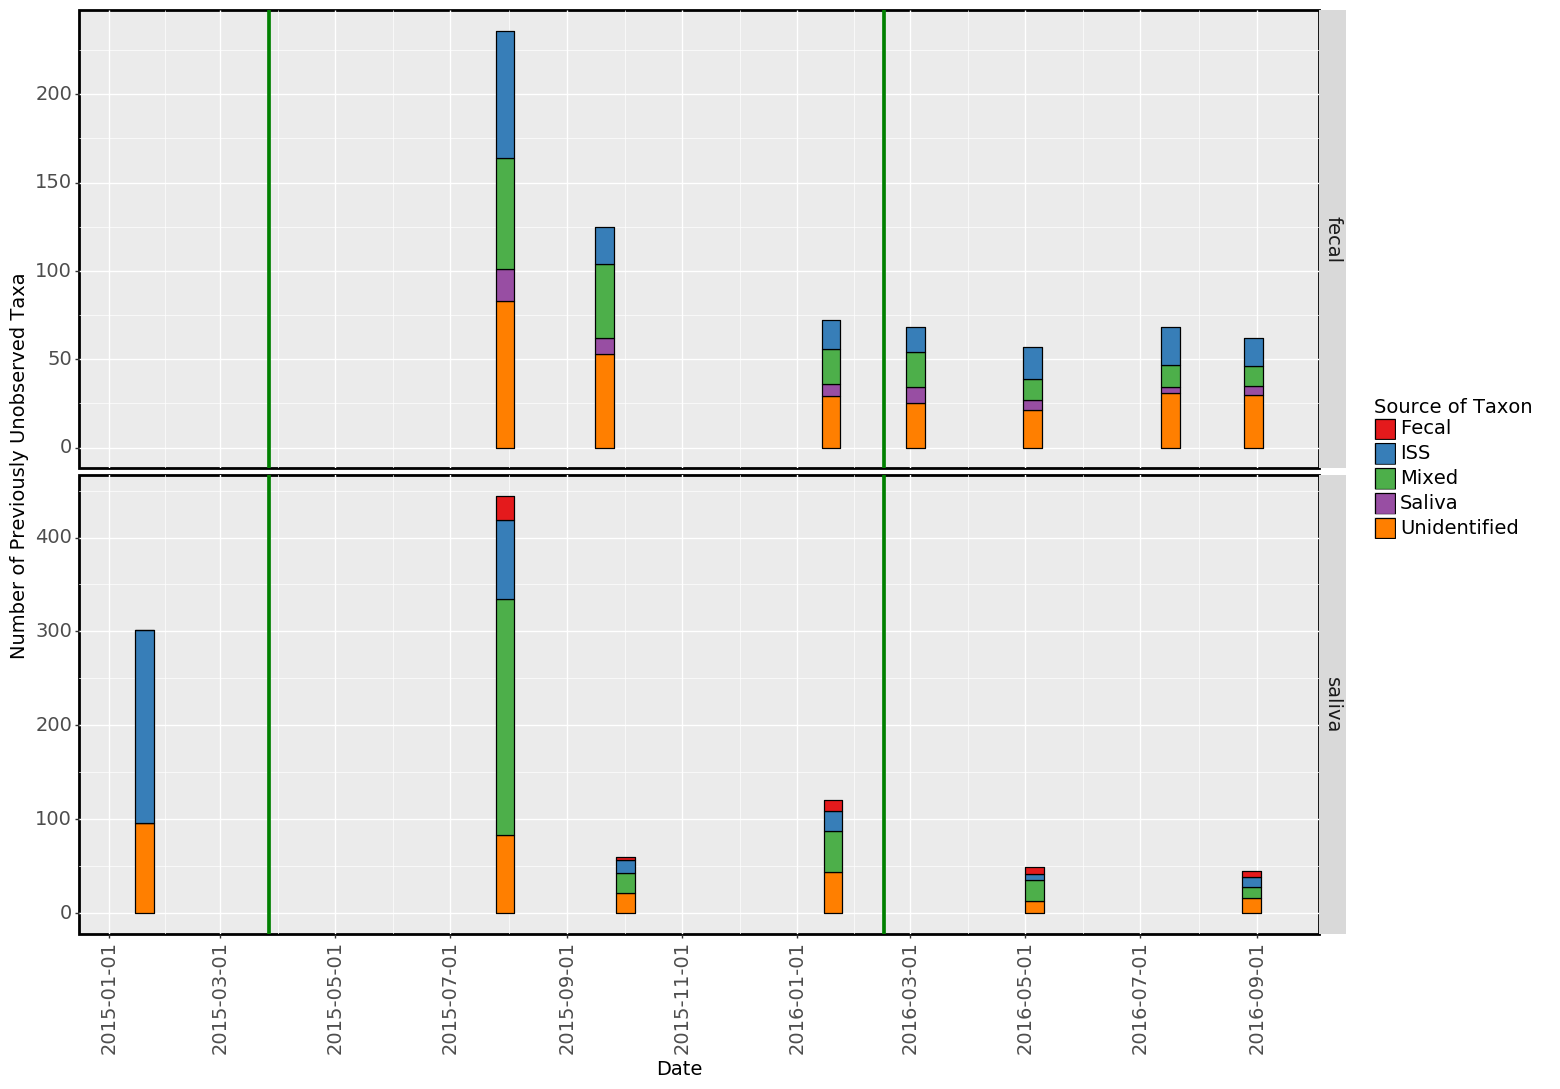
\includegraphics[width=0.99\textwidth]{figs/hr_taxa_sources.png}
%	\vspace{-20pt}
	\caption{\small{
	    This plot shows the number of taxa at each time point that were not observed at any previous timepoint for fecal and saliva samples from HR. The colors indicate the likely source of the new taxon if it was found previously in the saliva (for fecal samples, vice versa for saliva samples), the ISS, both (Mixed), or neither.
	}}
    \label{fig:hrtaxasource}
  \end{center}
%  \vspace{-20pt}
 % \vspace{1pt}
\end{figure}

\begin{figure}
  \begin{center}
    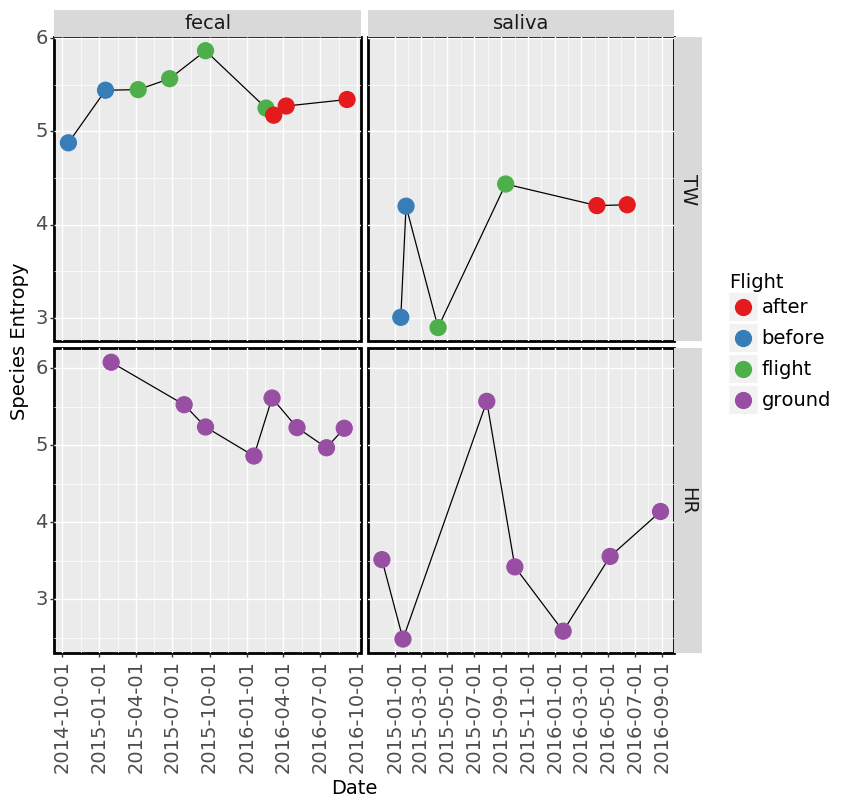
\includegraphics[width=0.99\textwidth]{figs/species_diversity.png}
%	\vspace{-20pt}
	\caption{\small{
	    Vertical shows species entropy (Shannon entropy of species relative abundances) for sample types in both twins.
	}}
    \label{fig:taxadiv}
  \end{center}
%  \vspace{-20pt}
 % \vspace{1pt}
\end{figure}

\begin{figure}
  \begin{center}
    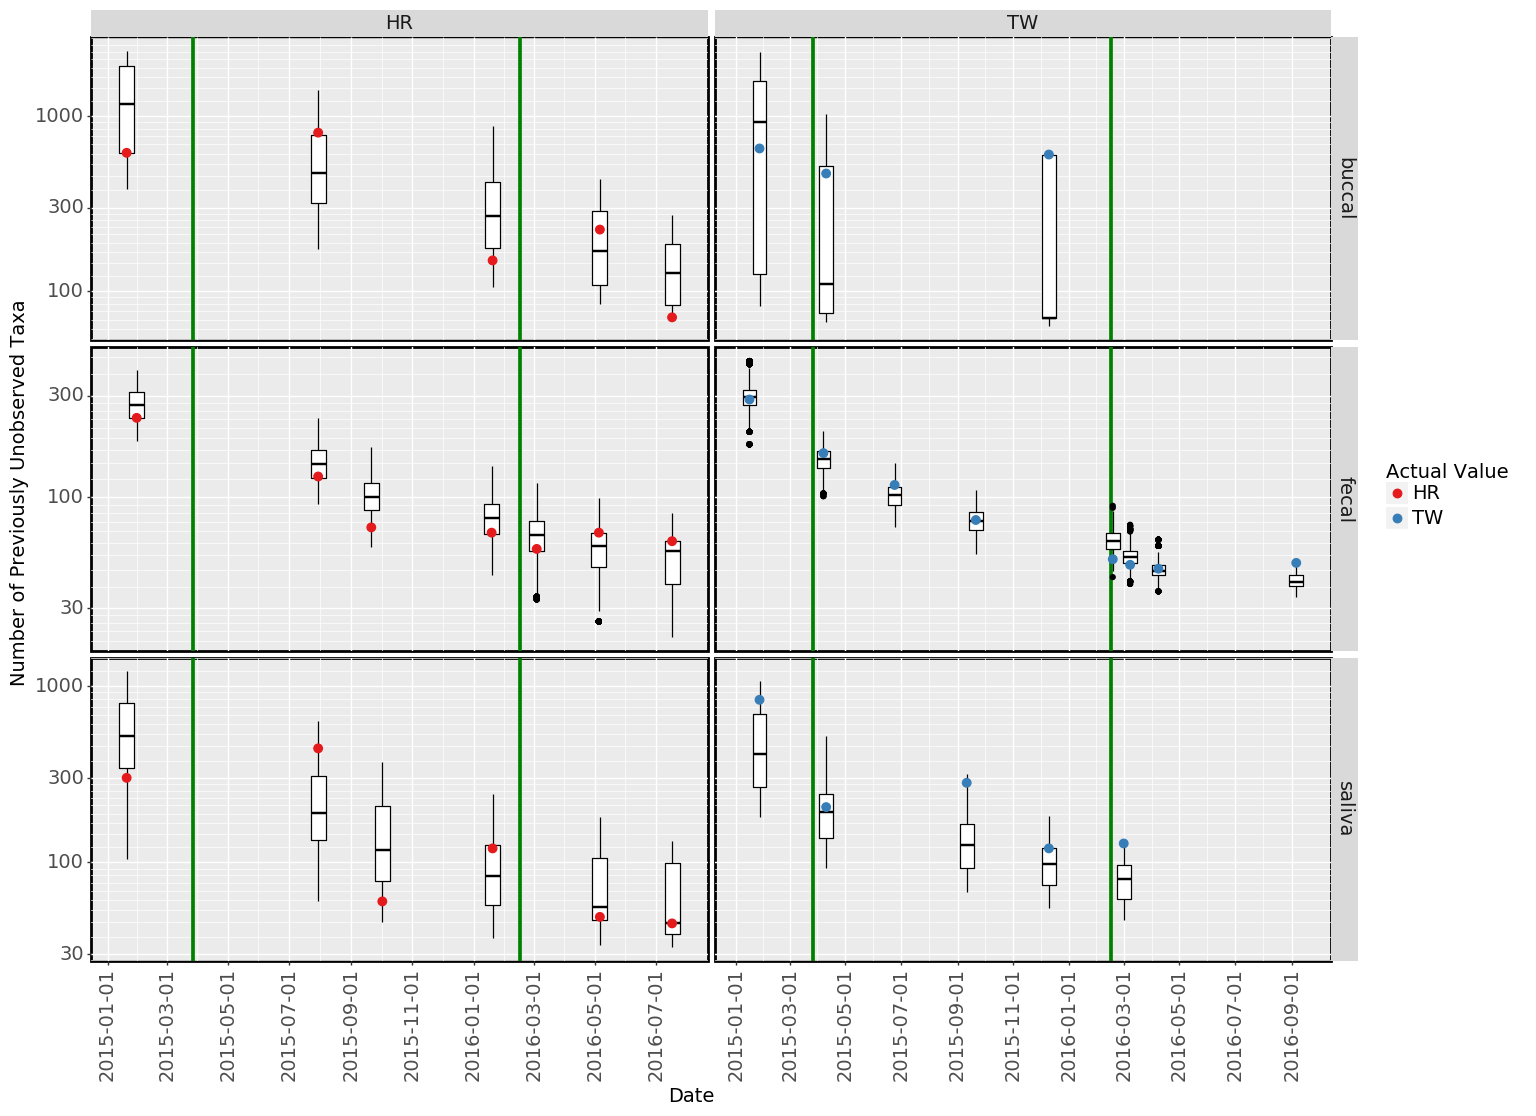
\includegraphics[width=0.99\textwidth]{figs/twins_taxa_flux.png}
%	\vspace{-20pt}
	\caption{\small{
	    This plot shows the number of taxa at each time point that were not observed at any previous timepoint. The first timepoint is omitted from the plot since no taxa had been previously observed. Boxplots indicate an artificial reference distribution generated by randomly permuting timestamps. Red and blue dots indicate actual values.
	}}
    \label{fig:taxaflux}
  \end{center}
%  \vspace{-20pt}
 % \vspace{1pt}
\end{figure}

\begin{figure}
  \begin{center}
    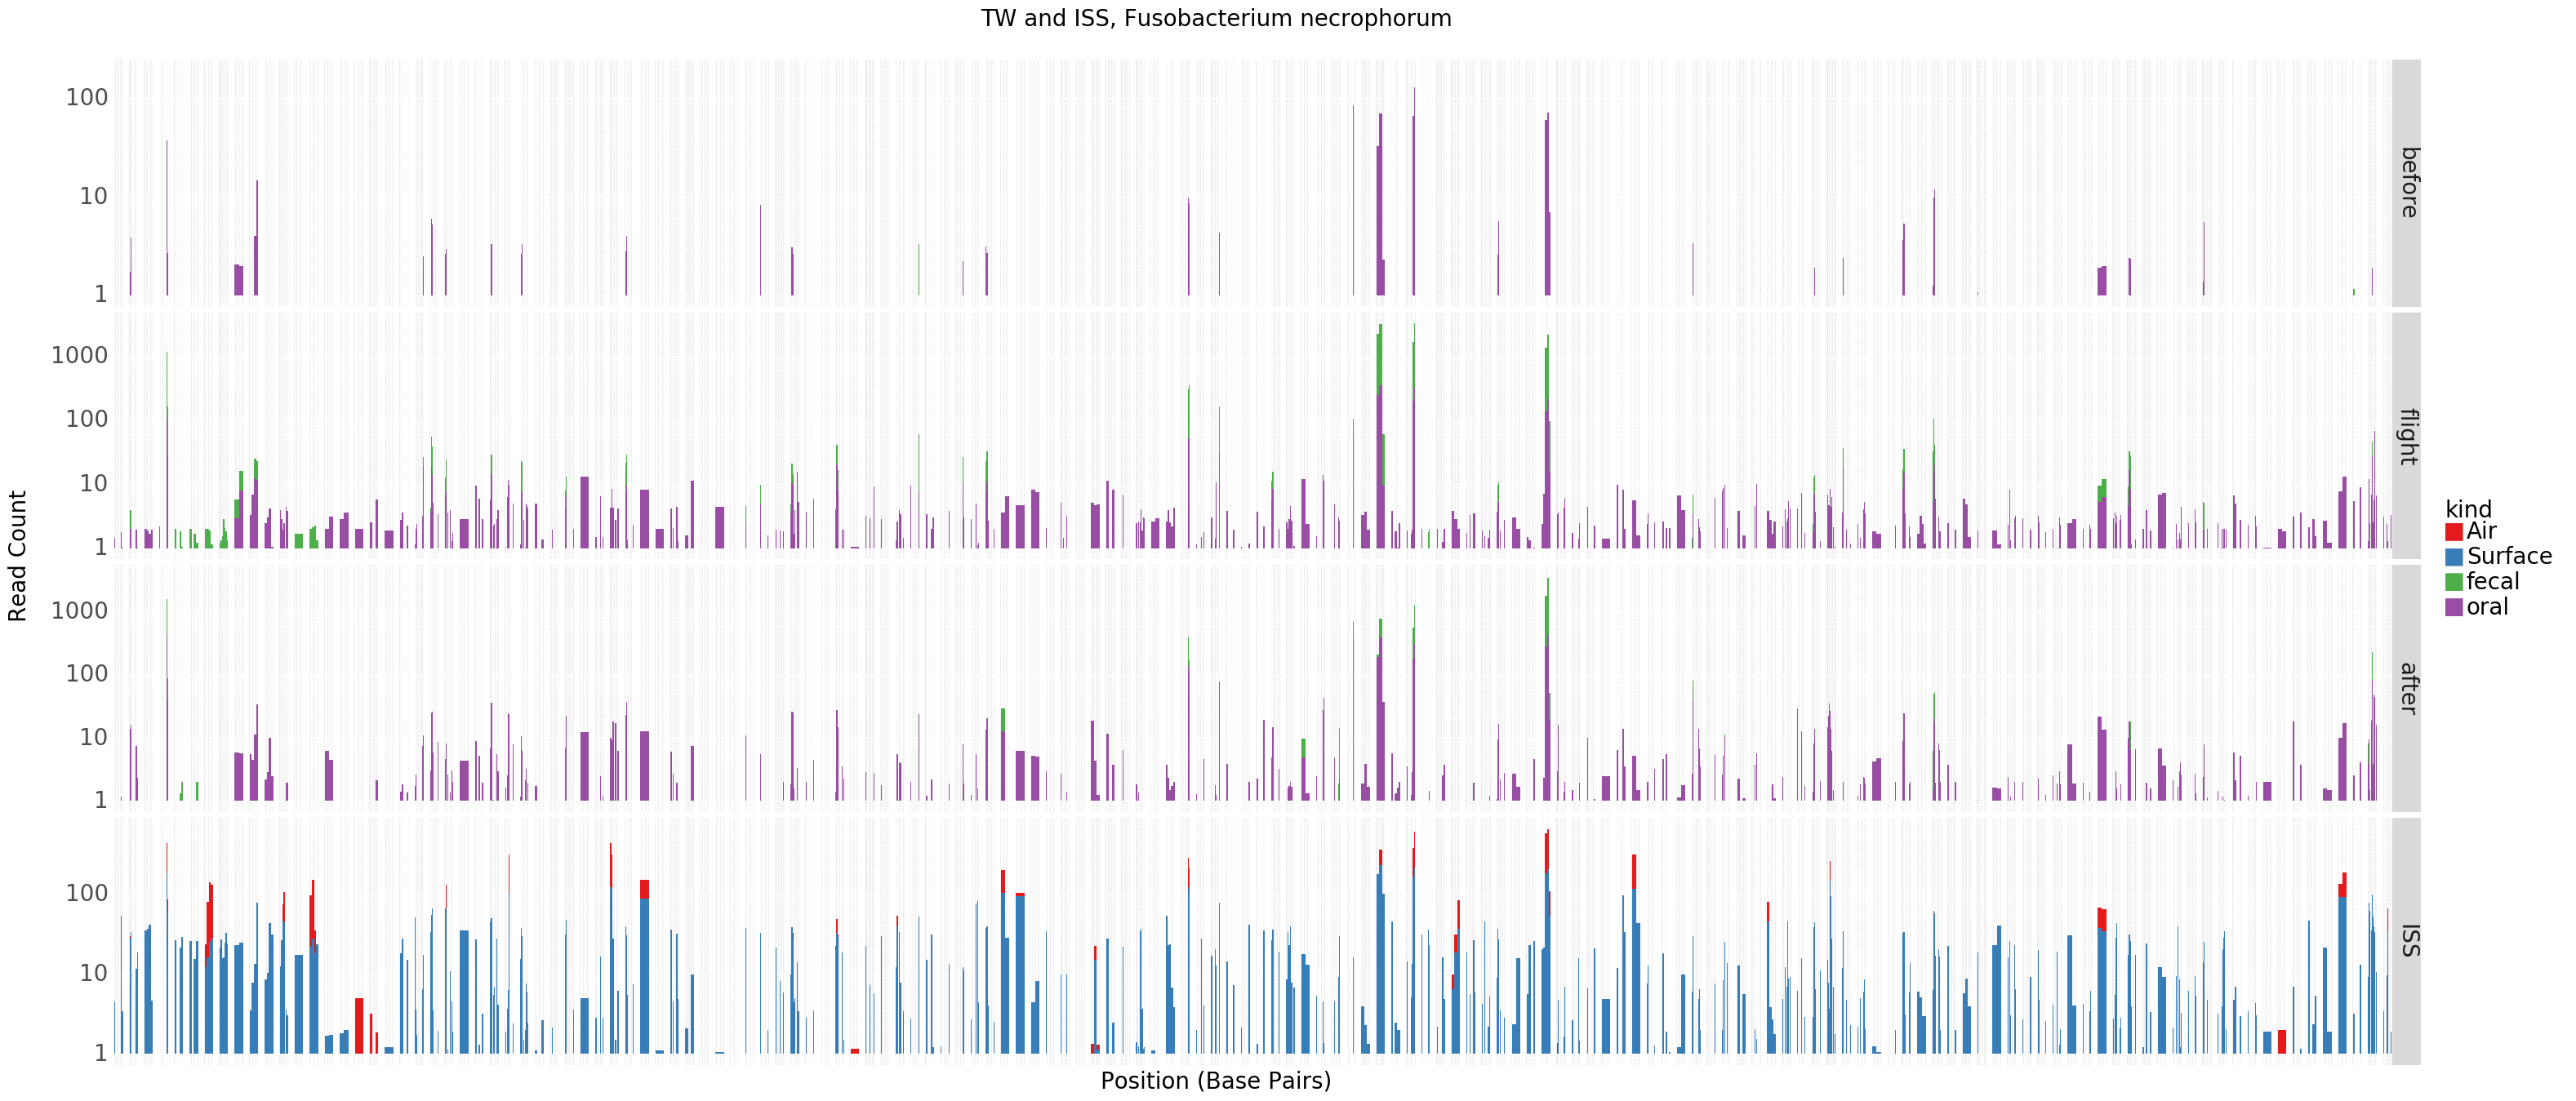
\includegraphics[width=0.99\textwidth]{figs/f_necro_read_recruit.png}
%	\vspace{-20pt}
	\caption{\small{
	    Rows show consolidated samples from before, during and after flight (or from the ISS at any point) from TW. Columns represent all available contigs for taxon. Colored bars represent 100bp covered, on average, at the specified read depth. A number of contigs are only covered in TW during and after flight.
	}}
    \label{fig:fnecro}
  \end{center}
%  \vspace{-20pt}
 % \vspace{1pt}
\end{figure}


\section{Transfer Case Study: Serratia Proteamaculans}

\paragraph{SP is a candidate persistent transfer}

\begin{figure}
  \begin{center}
    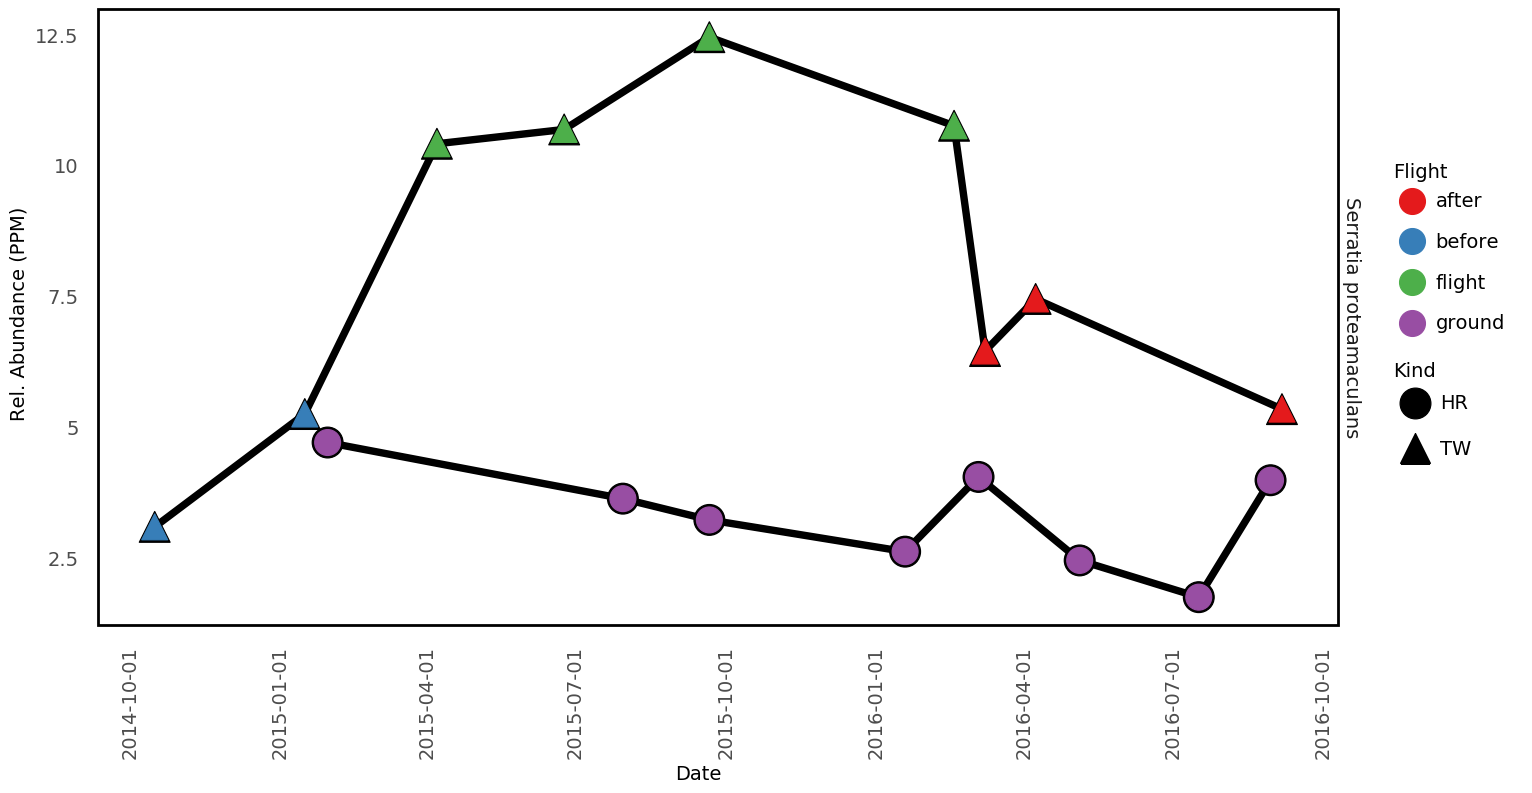
\includegraphics[width=0.99\textwidth]{figs/sp_abundance.png}
%	\vspace{-20pt}
	\caption{\small{
	    Relative abundance of \textit{Serratia proteamaculans} in fecal samples from TW and HR. Relative abundance is given in units of parts per million.
	}}
    \label{fig:abundance}
  \end{center}
%  \vspace{-20pt}
 % \vspace{1pt}
\end{figure}

We identified SP as a candidate persistent transfer, a species that was found in ISS environmental samples and was significantly more abundant in peri and post flight fecal samples from TW than other fecal samples. As a whole SP was only found at low levels in fecal samples in TW pre-flight, was significantly more abundant during flight, and dropped to an intermediate level after flight (Figure \ref{fig:abundance}). No major variation in abundance was observed for the control twin HR. SP was roughly uniformly abundant in the saliva before during and after flight.

\paragraph{Regions of the SP genome are found in TW fecal samples only after arrival at the ISS}

\begin{figure}
  \begin{center}
    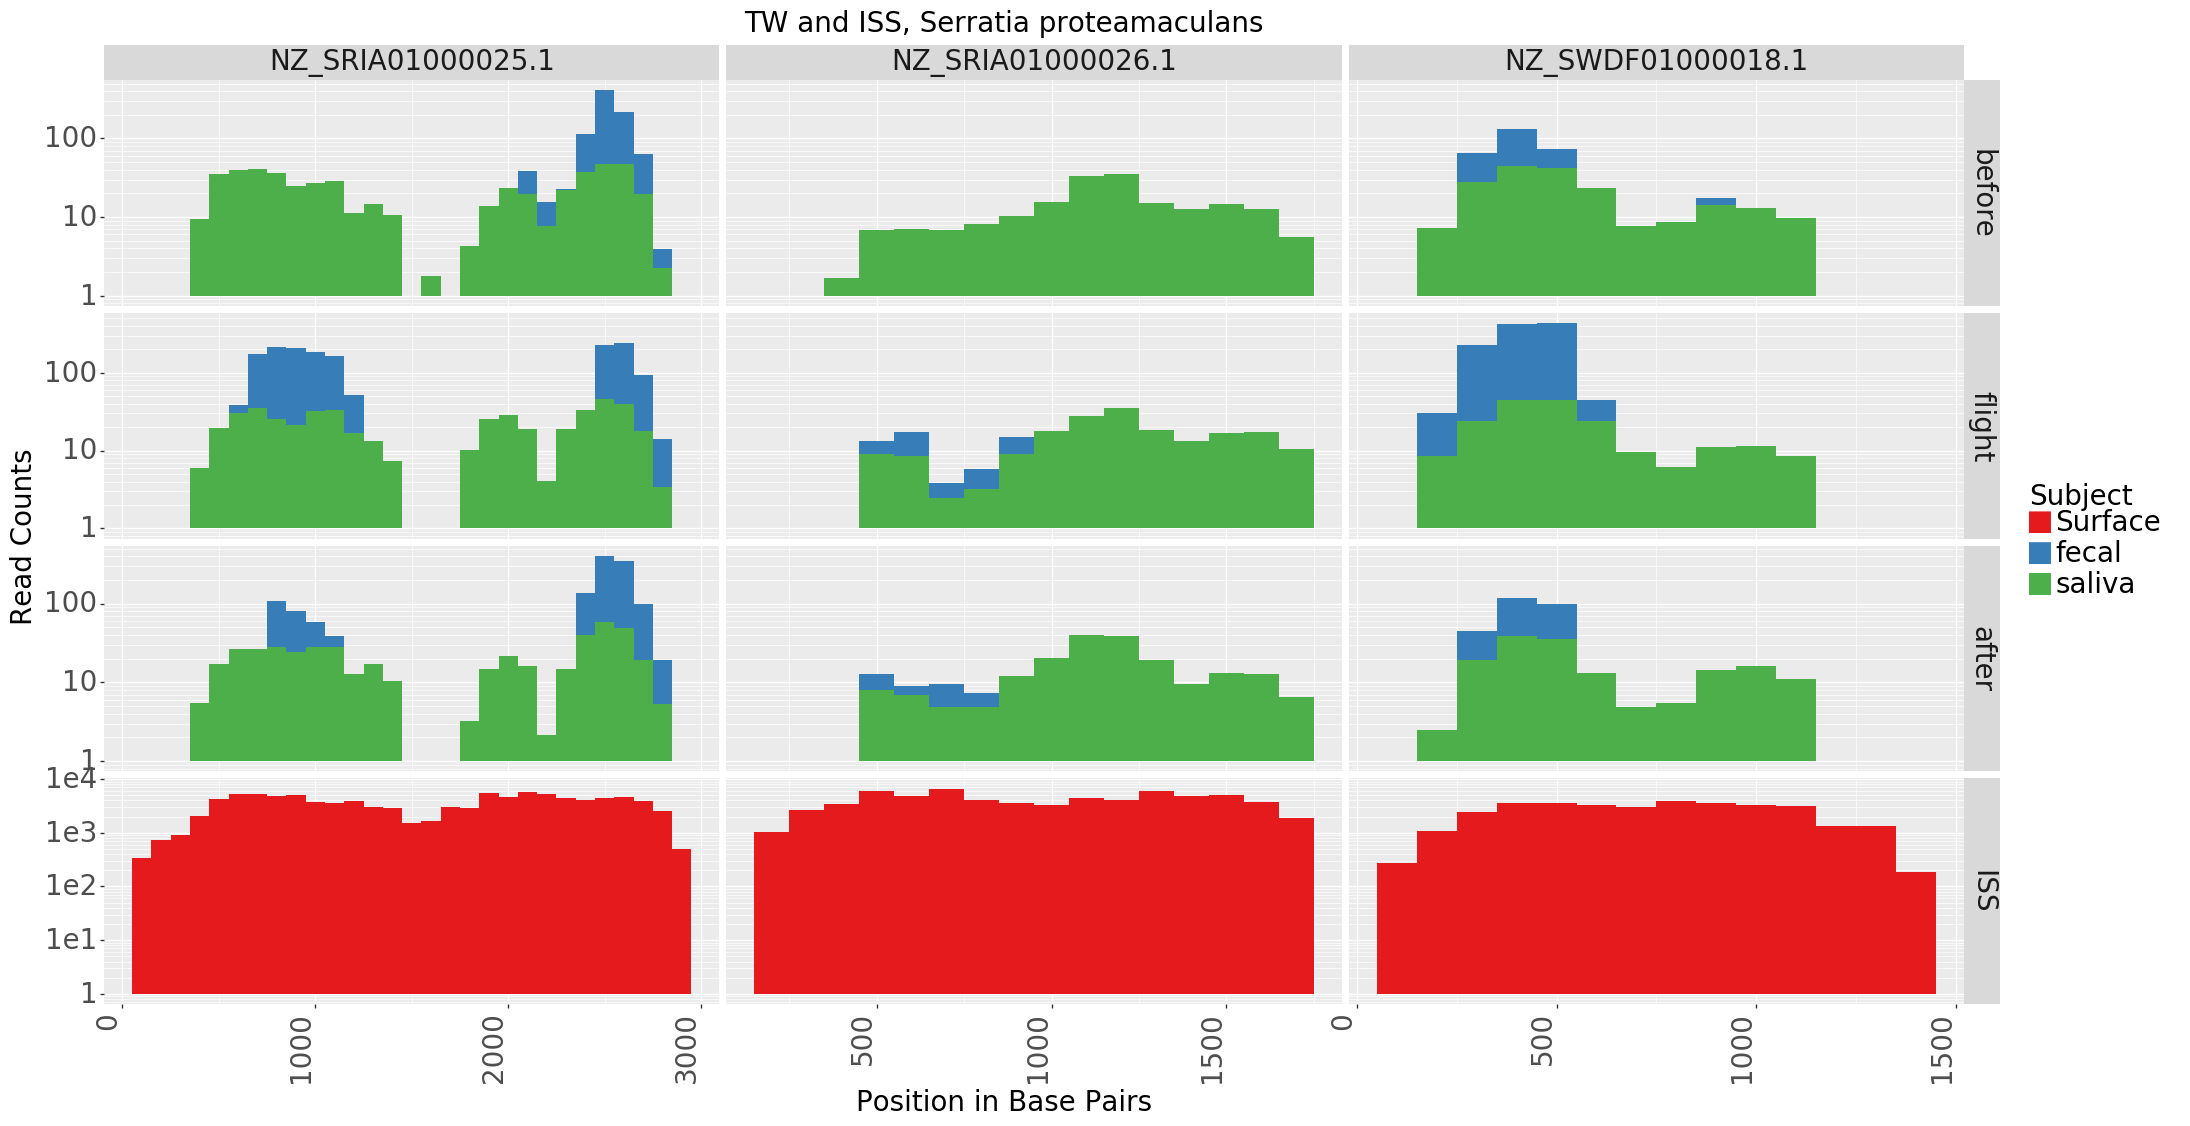
\includegraphics[width=0.99\textwidth]{figs/sprota_read_recruit.png}
%	\vspace{-20pt}
	\caption{\small{
	    Coverage of candidate persistent transfer regions of the \textit{Serratia proteamaculans} genome.
	}}
    \label{fig:sprota}
  \end{center}
%  \vspace{-20pt}
 % \vspace{1pt}
\end{figure}

We identified regions of the SP genome which appeared in fecal samples after TW was on board the ISS. We found three such regions totaling about 1.5kbp. The abundance of these regions roughly matched the overall pattern seen for SP. Very low or undetectable pre-flight, a high during flight, and an intermediate level post flight (Figure \ref{fig:sprota}). These regions were all well covered from ISS environmental samples.

Total coverage of the SP genome in TW from all available samples 29.2kbp. Before flight 8.9kbp was covered, during 17.2kbp and after 19.0kbp. However some of these regions were either quite small or not covered in both peri and post flight. As such 1.5kbp represents a reasonable fraction of the amount of SP genome covered in TW but should only be interpreted as evidence for the transfer of particular genes. 


\subsection{SNPs in post-arrival regions match a secondary environmental strain}

We analyzed one of the above regions (of about 250bp) for SNPs (Figure \ref{fig:bcsources}A) and identified SNPs in samples from TW which were either not found in the ISS environment or were found at different proportions. We identified 9 SNPs in this region during flight that were found in fewer than half of the ISS environmental samples. Of these 9 SNPs 6 were found after the conclusion of flight. We note that all of these 9 SNPs were found in ISS environmental samples at some proportion.

Next we used the SNP clustering technique described in the methods to determine if the 9 peri-flight SNPs we identified could come from the same strain. We identified corresponding groups of 8 SNPs in TW and 9 SNPs in the ISS environment. The 8 SNP group in TW included 8 out of the 9 peri-flight SNPs. The 9 SNP group from the ISS environment included these 8 SNPs as well as one SNP not identified in TW. This leads us to the conclusion that the strain found in TW likely represented a secondary strain in the ISS environment. 
